%
%  This is part of the SIGI.
%  Copyright (C) 2008 Interlegis
%  See the file relatorio.tex for copying conditions.
%

\section{Anexos}
\label{sec:anexos}

\subsection{Visão Geral}
\label{sec:a2}
O \textbf{SIGI} é um projeto para um Sistema de Informações Gerenciais do
\href{http://www.interlegis.gov.br/}{Interlegis}, escrito na linguagem de
programação \href{http://www.python.org}{Python} com o framework para
desenvolvimento web \href{http://www.djangoproject.org}{Django}.
\begin{description}
%[visit_definition_list_item]
\item[{Página do projeto}:] %[visit_definition]

\href{http://colab.interlegis.gov.br/wiki/ProjetoSigi}{http://colab.interlegis.gov.br/wiki/ProjetoSigi}

%[depart_definition]
%[depart_definition_list_item]
\end{description}


%___________________________________________________________________________

\hypertarget{caracter-sticas}{}
\pdfbookmark[0]{Características}{caracter-sticas}
\subsubsection*{Características}

Lista das principais características do SIGI:
\begin{itemize}
\item {} 
Serviço web cliente/servidor, podendo ser disponibilizado tanto na
internet quanto na intranet;

\item {} 
Multi-plataforma;

\item {} Baseia-se na interface de administração nativa do Django
  (\verb|django.contrib.admin|, maiores informações em
  \href{http://docs.djangoproject.com/en/dev/ref/contrib/admin/}{http://docs.djangoproject.com/en/dev/ref/contrib/admin/});

\item {} 
Gerencia convênios, equipamentos e inventários, serviços prestados e
composição de Mesas Diretoras das Casas Legislativas;

\item {} 
Autenticação no sistema baseada em usuários e grupos, com perfis
diferentes;

\item {} 
Emissão de relatórios.

\end{itemize}


%___________________________________________________________________________

\hypertarget{requisitos-b-sicos-de-software}{}
\pdfbookmark[0]{Requisitos básicos de software}{requisitos-b-sicos-de-software}
\subsubsection*{Requisitos básicos de software}
\begin{itemize}
\item {} 
Python {\textgreater}= 2.4 {\textless} 3.0

\item {} 
Django 1.0

\end{itemize}


%___________________________________________________________________________

\hypertarget{licen-a-de-uso}{}
\pdfbookmark[0]{Licença de uso}{licen-a-de-uso}
\subsubsection*{Licença de uso}

O SIGI é disponibilizado como
\href{http://pt.wikipedia.org/wiki/Software_Livre}{software livre},
isto significa que você pode redistribuí-lo e/ou modifica-lo dentro
dos termos da Licença Pública Geral GNU (GPL) como publicada pela
Fundação do Software Livre (FSF); na versão 3 da Licença, ou (na sua
opinião) em qualquer versão mais recente.

Veja o arquivo \texttt{LEIA-ME} para maiores informações a respeito das
condições de cópia e redistribuição.

\subsection{Organização do sistema}
\label{sec:org}

\subsubsection{Listagem do conteúdo dos diretórios}
\verbatiminput{../arquivos/tree.txt}

\subsubsection{Descrição dos arquivos e diretórios}
\begin{description}
\item[COPYING:] Arquivo com a licença do sistema (GPLv3).

\item[LEIA-ME/README:] Contém informações do sistema, nota de
  copyright e instruções de instalação.

\item[devel.db:] Base de dados SQLite utilizada para desenvolvimento
  do sistema.

\item[docs/:] Diretório com toda documentação escrita para o sistema
  (relatórios, manual de instalação, casos de uso, esquema de base de
  dados, etc).

\item[etc/:] Diretório com arquivos variados: configuração do Apache,
  \textit{patchs} de códigos, etc.

\item[media/:] Diretório com arquivos estáticos e de mídia do sistema
  (imagens, CSS, javascripts).

\item[sigi/:] Pacote Python do sistema.

\item[sigi/admin/:] Pacote de código relacionado com a aplicação
  \verb|admin| do Django (\verb|django.contrib.admin|).

\item[sigi/apps/:] Pacote de aplicações do sistema, maiores
  informações na Seção \ref{sec:apps}.

\item[sigi/settings.py:] Configurações padrões do sistema.

\item[sigi/local\_settings.template:] Exemplo de configurações locais
  do sistema (pertinentes à instalação). Deverá ser copiado para
  \verb|sigi/local_settings.py| para sua utilização.

\item[sigi/locale/:] Diretório com localização local do projeto.

\item[sigi/manage.py:] Script de gerenciamento do projeto, gerado pelo
  framework Django.

\item[sigi/templates/:] Diretório com templates HTML do Django.

\item[sigi/urls.py:] Modulo de configuração de URLs.
\end{description}

\subsubsection{Descrição das aplicações}
\label{sec:apps}
O SIGI é composto de algumas aplicações Django, cada uma com um
propósito bem definido.

Uma aplicação Django é um pacote Python modular, podendo ser
reaproveitado em outros projetos.

Algumas aplicações possuem algum nível de relacionamento com as
outras.

Segue descrição de cada aplicação:

\begin{description}
\item[sigi.apps.casas:]
  Gerência de Casas Legislativas.

\item[sigi.apps.contatos:]
  Gerência de Contatos do Interlegis com Casas Legislativas,
  fornecedores de equipamentos, serviços e etc.

\item[sigi.apps.convenios:]
  Convênios do Interlegis com as Casas Legislativas.

\item[sigi.apps.inventario:]
  Inventário de equipamentos disponibilizados pelo Interlegis para as
  Casas Legislativas.

\item[sigi.apps.mesas:]
  Composição das Mesas Diretoras das Casas Legislativas.

\item[sigi.apps.parlamentares:]
  Gerência de Parlamentares.

\item[sigi.apps.servicos:]
  Serviços prestados às Casas Legislativas conveniadas ao Interlegis.
\end{description}

\subsubsection{Relacionamento entre as aplicações}
\label{sec:rel}

A Figura \ref{fig:apps} demonstra o relacionamento entre as
aplicações e seus \emph{models}.

Uma seta direcional representa uma relação \textit{muitos para
  um}. Uma seta bidirecional representa uma relação \textit{muitos
  para muitos}.

A seta pontilhada representa uma relação genérica, como descrito na
documentação do Django:\\
http://docs.djangoproject.com/en/dev/ref/contrib/contenttypes/\#id1

\begin{figure}[p]
  \centering
  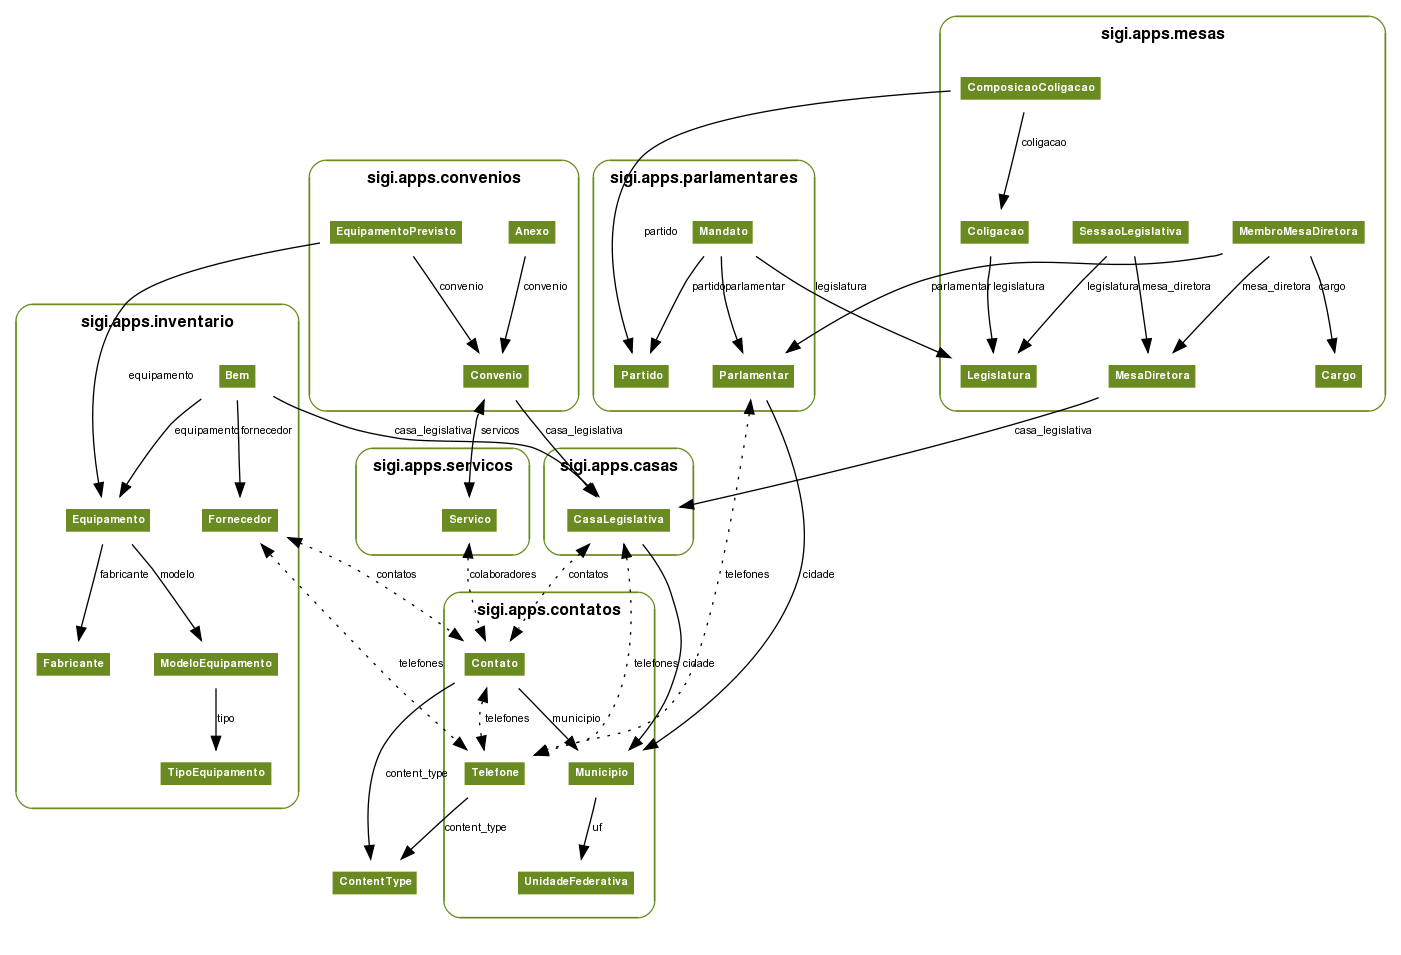
\includegraphics[angle=90,width=130mm]{../imagens/apps.png}
  \caption{Relacionamento entre as aplicações}
  \label{fig:apps}
\end{figure}

\subsection{Casos de Uso}
\label{sec:casos}

Esta seção descreve a utilização do sistema através de \emph{Casos de
  Uso}, representando os principais atores e suas interações com o
sistema.

Os Casos de Uso servem de auxílio à compreensão dos usuários quanto à
implementação e uso do sistema.

\subsubsection{Casos de Uso do SIGI}
A Figura \ref{fig:casos} apresenta os Casos de Uso do SIGI de maneira
simplificada.

\begin{figure}[h]
  \centering
  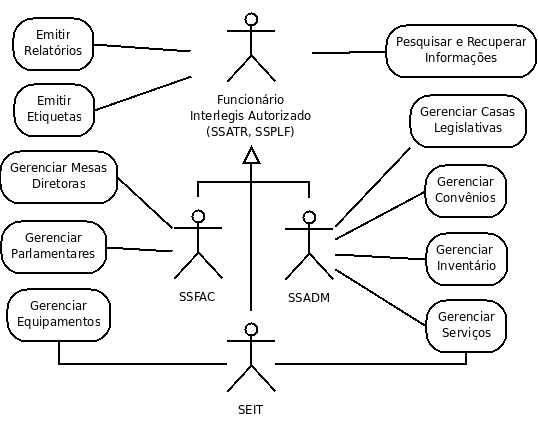
\includegraphics[width=120mm]{../imagens/casosdeuso.png}
  \caption{Casos de Uso}
  \label{fig:casos}
\end{figure}

\paragraph{Descrição dos Atores}
\begin{description}
\item[Funcionário Interlegis Autorizado:] usuário apenas com
  atribuições de leitura no sistema. Inclui pessoal da Subsecretaria
  de Apoio Técnico e Relações Institucionais (SSATR) e Subsecretaria
  de Planejamento e Fomento (SSPLF).
\item[SSFAC:] Subsecretaria de Formação e Atendimento à Comunidade do
  Legislativo.
\item[SSADM:] Subsecretaria de Administração.
\item[SEIT:] Serviço de Infra-estrutura Tecnológica.
\end{description}

\paragraph{Descrição das Atividades}
\begin{description}
\item[Emitir Relatórios:] consiste em obter informações e emitir
  relatórios de diversas partes do sistema.
\item[Emitir Etiquetas:] consiste em obter informações e emitir
  etiquetas de algumas partes do sistema.
\item[Pesquisar e Recuperar Informações:] habilidades de pesquisa e
  obtenção de informações da base de dados do sistema.
\item[Gerenciar Mesas Diretoras:] consiste em inserir, atualizar e
  remover \emph{Mesas Diretoras}, \emph{Sessões Legislativas} e
  modificar a \emph{Composição das Mesas Diretoras}.
\item[Gerenciar Parlamentares:] consiste em inserir, atualizar e
  remover \emph{Parlamentares} e \emph{Partidos}.
\item[Gerenciar Equipamentos:] consiste em inserir, atualizar e
  remover \emph{Equipamentos} e \emph{Fornecedores}.
\item[Gerenciar Casas Legislativas:] consiste em inserir, atualizar e
  remover \emph{Casas Legislativas}.
\item[Gerenciar Convênios:] consiste em inserir, atualizar e remover
  \emph{Convênios}.
\item[Gerenciar Inventário:] consiste em atualizar o \emph{Inventário}
  das Casas Legislativas.
\item[Gerenciar Serviços:] consiste em inserir, atualizar e remover
  \emph{Serviços} prestados às Casas Legislativas.
\end{description}

\subsection{Modelo de dados}
\label{sec:modelo}

\subsubsection{Aplicação sigi.apps.casas (figura \ref{fig:casas})}
\begin{figure}[h!]
  \centering
  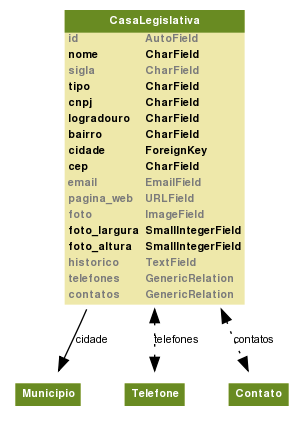
\includegraphics[width=60mm]{../imagens/casas.png}
  \caption{Diagrama de Classes da aplicação sigi.apps.casas}
  \label{fig:casas}
\end{figure}

\subsubsection{Aplicação sigi.apps.contatos (figura \ref{fig:contatos})}
\begin{figure}[h!]
  \centering
  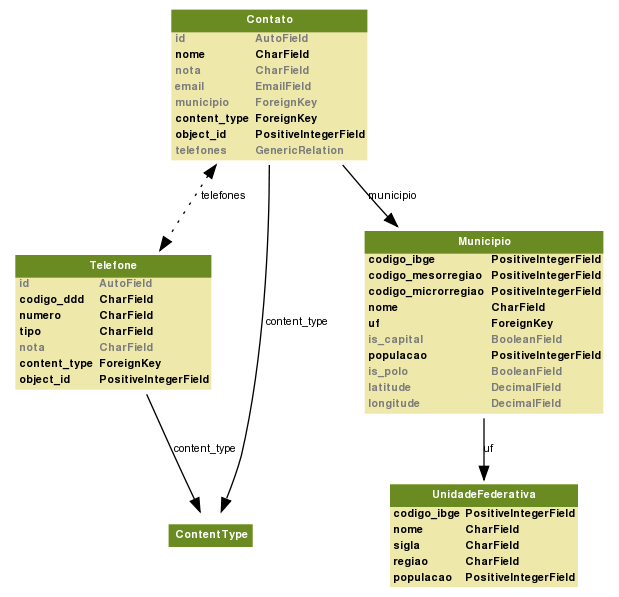
\includegraphics[width=120mm]{../imagens/contatos.png}
  \caption{Diagrama de Classes da aplicação sigi.apps.contatos}
  \label{fig:contatos}
\end{figure}

\subsubsection{Aplicação sigi.apps.convenios (figura \ref{fig:convenios})}
\begin{figure}[h!]
  \centering
  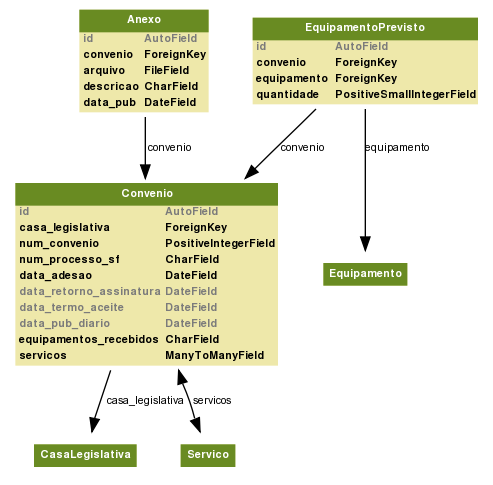
\includegraphics[width=100mm]{../imagens/convenios.png}
  \caption{Diagrama de Classes da aplicação sigi.apps.convenios}
  \label{fig:convenios}
\end{figure}

\subsubsection{Aplicação sigi.apps.inventario (figura \ref{fig:inventario})}
\begin{figure}[h!]
  \centering
  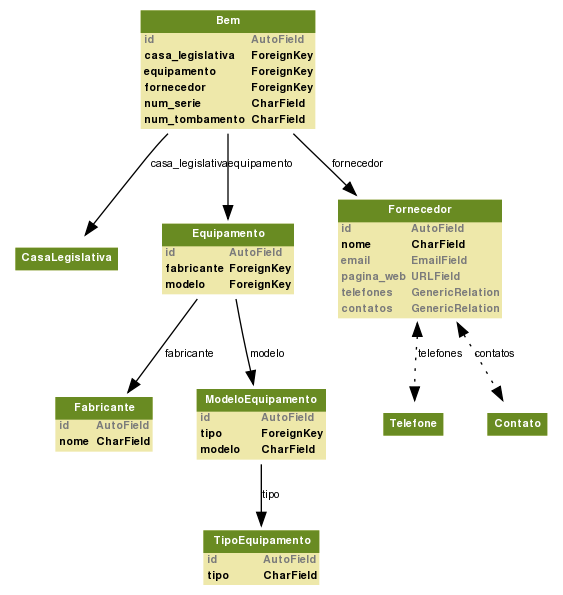
\includegraphics[width=120mm]{../imagens/inventario.png}
  \caption{Diagrama de Classes da aplicação sigi.apps.inventario}
  \label{fig:inventario}
\end{figure}

\subsubsection{Aplicação sigi.apps.mesas (figura \ref{fig:mesas})}
\begin{figure}[h!]
  \centering
  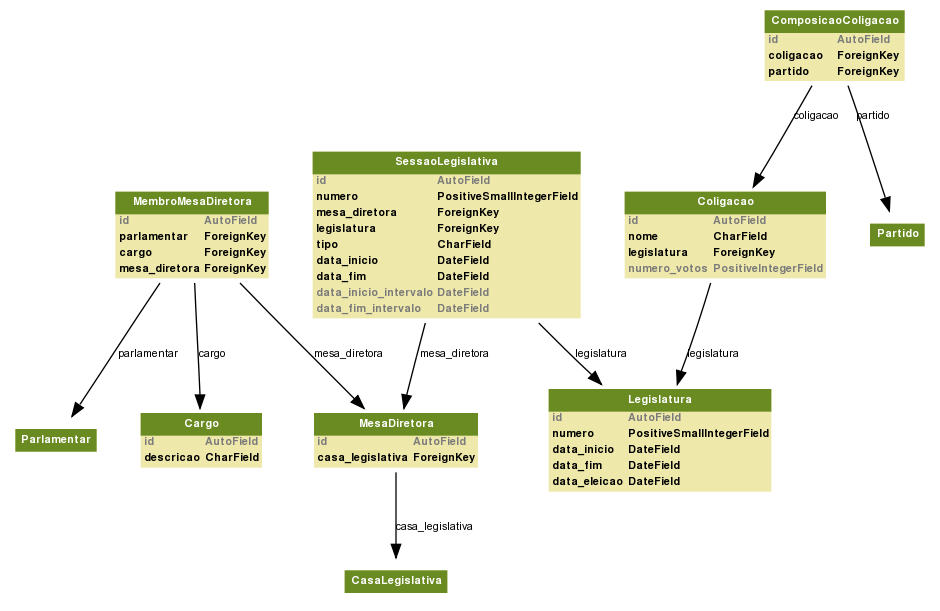
\includegraphics[width=145mm]{../imagens/mesas.png}
  \caption{Diagrama de Classes da aplicação sigi.apps.mesas}
  \label{fig:mesas}
\end{figure}

\subsubsection{Aplicação sigi.apps.parlamentares (figura \ref{fig:parlamentares})}
\begin{figure}[h!]
  \centering
  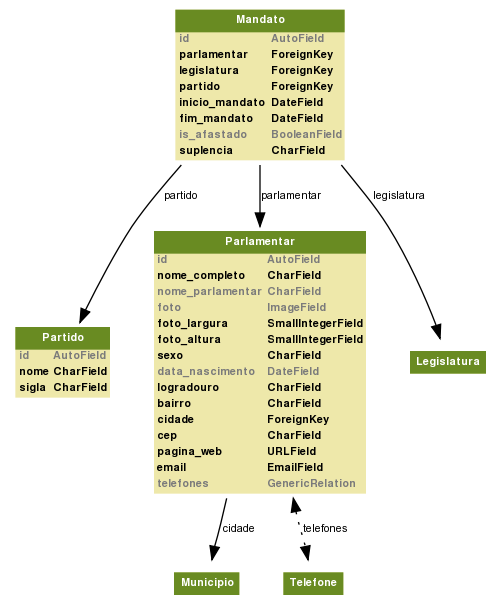
\includegraphics[width=100mm]{../imagens/parlamentares.png}
  \caption{Diagrama de Classes da aplicação sigi.apps.parlamentares}
  \label{fig:parlamentares}
\end{figure}

\subsubsection{Aplicação sigi.apps.servicos (figura \ref{fig:servicos})}
\begin{figure}[h!]
  \centering
  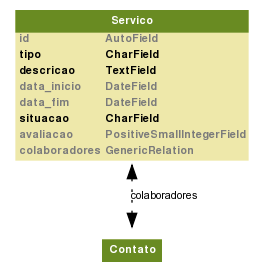
\includegraphics[width=60mm]{../imagens/servicos.png}
  \caption{Diagrama de Classes da aplicação sigi.apps.servicos}
  \label{fig:servicos}
\end{figure}

\subsection{Esquema de dados}
\label{sec:esquema}

Nesta seção estão descritos os esquemas de criação das entidades e de
seus relacionamentos do banco de dados \emph{SQL} para cada aplicação
do SIGI.

\small
\subsubsection{Aplicação sigi.apps.casas}
\verbatiminput{../arquivos/casas.sql}

\subsubsection{Aplicação sigi.apps.contatos}
\verbatiminput{../arquivos/contatos.sql}

\subsubsection{Aplicação sigi.apps.convenios}
\verbatiminput{../arquivos/convenios.sql}

\subsubsection{Aplicação sigi.apps.inventario}
\verbatiminput{../arquivos/inventario.sql}

\subsubsection{Aplicação sigi.apps.mesas}
\verbatiminput{../arquivos/mesas.sql}

\subsubsection{Aplicação sigi.apps.parlamentares}
\verbatiminput{../arquivos/parlamentares.sql}

\subsubsection{Aplicação sigi.apps.servicos}
\verbatiminput{../arquivos/servicos.sql}
\normalsize

\subsection{Manual de Instalação}
\label{sec:a3}
Este documento descreve como efetuar a instalação do Sistema de
Informações Gerenciais do Interlegis (SIGI). Os passos são baseados
nas distribuições GNU/Linux Debian e Ubuntu. Podem ser aplicados sem
dificuldades em outras distribuições, mas poderão sofrer alguma
adaptação.


%___________________________________________________________________________

\hypertarget{prepara-o-do-ambiente-para-a-instala-o}{}
\pdfbookmark[0]{Preparação do ambiente para a instalação}{prepara-o-do-ambiente-para-a-instala-o}
\subsubsection{Preparação do ambiente para a instalação}

Há dois tipos de instalação do SIGI, uma para desenvolvimento e outra
para produção.

Para ambas instalações, certifique-se que os seguintes softwares
estejam instalados em seu sistema:
\begin{itemize}
\item {} 
Python {\textgreater}= 2.4 {\textless} 3.0

\item {} 
Django 1.0

\end{itemize}

O Python pode ser instalado a partir do pacote \texttt{python} com uma
ferramenta de instalação de pacotes como o \texttt{apt-get} ou
\texttt{aptitude}.

Se a sua distribuição não possui o pacote \texttt{python-django}, para
o Django na versão 1.0, será necessário obter e configurar o mesmo
manualmente. A próxima seção traz mais detalhes para esta tarefa.


%___________________________________________________________________________

\hypertarget{instala-o-do-django}{}
\pdfbookmark[1]{Instalação do Django}{instala-o-do-django}
\subsubsection*{Instalação do Django}
O Django 1.0 pode ser obtido através da \href{http://www.djangoproject.com/download/}{página de download} do \href{http://www.djangoproject.com}{Django Project} via \emph{tarball} (\texttt{tar.gz}) ou via
Subversion (revisão 8961).


%___________________________________________________________________________

\hypertarget{obtendo-e-instalando-o-django}{}
\pdfbookmark[2]{Obtendo e instalando o Django}{obtendo-e-instalando-o-django}
\subsubsection*{Obtendo e instalando o Django}
Primeiramente baixe o \href{http://www.djangoproject.com/download/1.0/tarball/}{tarball do Django 1.0} ou dê
\emph{checkout} na tag 1.0 disponível no repositório do Subversion do
projeto:
\begin{quote}{\ttfamily \raggedright \noindent
svn~checkout~http://code.djangoproject.com/svn/django/tags/releases/1.0/
}\end{quote}

Após isso será necessário colocar o pacote Python do \texttt{django}
(diretório \texttt{django} disponível dentro do diretório/tarball baixado)
no \emph{path} do Python.

Para saber quais são os diretórios que estão no path do Python,
execute em linha de comando:
\begin{quote}{\ttfamily \raggedright \noindent
python~-c~'import~sys;~print~sys.path'
}\end{quote}

Você tem opção de mover o pacote \texttt{django} para algum diretório
coberto pelo path ou adicionar um outro local no path utilizando a
variável de ambiente \texttt{PYTHONPATH} do usuário que rodará o sistema. O
formato do \texttt{PYTHONPATH} é o mesmo do \texttt{PATH} do sistema. Exemplo:
\begin{quote}{\ttfamily \raggedright \noindent
PYTHONPATH=/path/to/django:{\$}PYTHONPATH
}\end{quote}

De maneira simplificada, a instalação do Django é como a instalação de
qualquer outro pacote Python.


%___________________________________________________________________________

\hypertarget{preparando-o-ambiente-para-desenvolvimento}{}
\pdfbookmark[1]{Preparando o ambiente para desenvolvimento}{preparando-o-ambiente-para-desenvolvimento}
\subsubsection*{Preparando o ambiente para desenvolvimento}

Se você irá desenvolver o SIGI, é necessário possuir os seguintes
pacotes instalados em sua máquina:
\begin{itemize}
\item {} 
sqlite3, para SQLite 3;

\item {} 
python-pysqlite2, interface Python para SQLite 3.

\end{itemize}


%___________________________________________________________________________

\hypertarget{preparando-o-ambiente-para-produ-o}{}
\pdfbookmark[1]{Preparando o ambiente para produção}{preparando-o-ambiente-para-produ-o}
\subsubsection*{Preparando o ambiente para produção}

Para disponibilizar o SIGI em um ambiente para produção você
necessitará do MySQL Server ou PostgreSQL, ou qualquer outro Sistema
Gerenciador de Banco de Dados (SGBD) compatível com Django 1.0, e de
suas seguintes interfaces para Python, como os pacotes
\texttt{python-mysqldb} e \texttt{python-psycopg2} (respectivamente para MySQL e
PostgreSQL).

Será necessário também possuir o Apache ({\textgreater}= 2.2) instalado para
disponibilizar o sistema via HTTP, de forma cliente/servidor, ou outro
servidor web compatível com Python e WSGI (ou FastCGI).

Opcionalmente, você pode utilizar o servidor web Lighttpd para servir
os arquivos estáticos do sistema.

Você encontrará configurações para Apache com WSGI neste documento,
juntamente com instruções para configurar o SIGI com o banco de dados
escolhido.


%___________________________________________________________________________

\hypertarget{instala-o-e-configura-o-do-sigi}{}
\pdfbookmark[0]{Instalação e configuração do SIGI}{instala-o-e-configura-o-do-sigi}
\subsubsection{Instalação e configuração do SIGI}

O SIGI está disponível no \href{http://colab.interlegis.gov.br}{Colab},
um portal colaborativo para a gerência dos projetos de software do
\href{http://www.interlegis.gov.br}{Interlegis}.

A página do projeto SIGI no Colab pode ser acessada através do link
\href{http://colab.interlegis.gov.br/wiki/ProjetoSigi}{http://colab.interlegis.gov.br/wiki/ProjetoSigi}.


%___________________________________________________________________________

\hypertarget{obtendo-e-instalando-o-sigi}{}
\pdfbookmark[1]{Obtendo e instalando o SIGI}{obtendo-e-instalando-o-sigi}
\subsubsection*{Obtendo e instalando o SIGI}

Para baixar o SIGI, é necessário ter o Subversion instalado em sua
máquina (pacote \texttt{subversion}). Para \emph{checkout} do sistema via
Subversion, execute o comando abaixo:
\begin{verbatim}
svn checkout http://repositorio.interlegis.gov.br/SIGI/trunk/ \
  /path/to/SIGI
\end{verbatim}

Substitua \texttt{/path/to/SIGI} para o local onde deseja instalar o
SIGI. (Iremos considerar o diretório SIGI como a raiz do projeto
durante o restante deste documento.)


%___________________________________________________________________________

\hypertarget{configura-o-do-sigi}{}
\pdfbookmark[1]{Configuração do SIGI}{configura-o-do-sigi}
\subsubsection*{Configuração do SIGI}

Dentro da raiz do projeto, encontra-se um diretório de nome \texttt{sigi}
(pacote Python do projeto). Sua configuração padrão, se encontra no
arquivo \texttt{settings.py}.

Para alterar as configurações do projeto, é recomendado que copie o
arquivo \texttt{local{\_}settings.template} para \texttt{local{\_}settings.py} e
altere os parâmetros neste arquivo.


%___________________________________________________________________________

\hypertarget{instala-o-em-ambiente-para-desenvolvimento}{}
\pdfbookmark[1]{Instalação em ambiente para desenvolvimento}{instala-o-em-ambiente-para-desenvolvimento}
\subsubsection*{Instalação em ambiente para desenvolvimento}

As configurações padrão do projeto já estão direcionadas para um
ambiente de desenvolvimento e não exige demais configurações.

(Os comandos abaixo deverão ser executados dentro do diretório
\texttt{sigi}, onde se encontra o arquivo \texttt{manage.py}.)


%___________________________________________________________________________

\hypertarget{base-de-dados-em-ambiente-para-desenvolvimento}{}
\pdfbookmark[2]{Base de dados em ambiente para desenvolvimento}{base-de-dados-em-ambiente-para-desenvolvimento}
\subsubsection*{Base de dados em ambiente para desenvolvimento}

Antes de executar o projeto, é necessário preencher o banco de dados
com suas tabelas e valores padrão.

Considerando que possua o SQLite instalado, basta executar o comando
abaixo:
\begin{quote}{\ttfamily \raggedright \noindent
python~manage.py~syncdb
}\end{quote}


%___________________________________________________________________________

\hypertarget{execu-o-do-projeto-em-ambiente-para-desenvolvimento}{}
\pdfbookmark[2]{Execução do projeto em ambiente para desenvolvimento}{execu-o-do-projeto-em-ambiente-para-desenvolvimento}
\subsubsection*{Execução do projeto em ambiente para desenvolvimento}

Para rodar o SIGI, execute em linha de comando:
\begin{quote}{\ttfamily \raggedright \noindent
python~manage.py~runserver
}\end{quote}

O projeto poderá ser acessado através do endereço
\href{http://127.0.0.1:8000/}{http://127.0.0.1:8000/}.


%___________________________________________________________________________

\hypertarget{instala-o-em-ambiente-para-produ-o}{}
\pdfbookmark[1]{Instalação em ambiente para produção}{instala-o-em-ambiente-para-produ-o}
\subsubsection*{Instalação em ambiente para produção}

Para instalar o SIGI em ambiente para produção, devemos configurar um
Sistema Gerenciador de Banco de Dados (SGBD), o qual armazenará os
dados do sistema, e configurar um servidor HTTP, como o Apache, para
disponibilizar o sistema na web.


%___________________________________________________________________________

\hypertarget{configura-o-do-sgdb}{}
\pdfbookmark[2]{Configuração do SGDB}{configura-o-do-sgdb}
\subsubsection*{Configuração do SGDB}

Modifique em seu \texttt{local{\_}settings.py} as variáveis
\texttt{DATABASE{\_}ENGINE}, \texttt{DATABASE{\_}NAME}, \texttt{DATABASE{\_}USER},
\texttt{DATABASE{\_}PASSWORD}, \texttt{DATABASE{\_}HOST} e \texttt{DATABASE{\_}PORT} de acordo
com o banco de dados disponibilizado para o SIGI.

Em \texttt{DATABASE{\_}ENGINE}, suas opções são \texttt{postgresql{\_}psycopg2},
\texttt{postgresql}, \texttt{mysql}, \texttt{sqlite3} ou \texttt{ado{\_}mssql}.

Após isso, é necessário preencher o banco de dados
com suas tabelas e valores padrão. Para tal, execute em linha de
comando:
\begin{quote}{\ttfamily \raggedright \noindent
python~manage.py~syncdb
}\end{quote}


%___________________________________________________________________________

\hypertarget{configura-o-do-servidor-web-apache-com-wsgi}{}
\pdfbookmark[2]{Configuração do servidor web Apache com WSGI}{configura-o-do-servidor-web-apache-com-wsgi}
\subsubsection*{Configuração do servidor web Apache com WSGI}

Exemplos de configurações, de um \texttt{VirtualHost}, estão disponíveis no
diretório \texttt{etc/apache/} dentro do diretório raiz do projeto
(\texttt{SIGI/}).

%
% Local variables:
%   mode: flyspell
%   TeX-master: "relatorio.tex"
% End:
%
